% Owner: member A. Numbers come from outputs/*/metrics.json via
% src/resource_table.py and from src/tfidf_dim_study.py. Rows marked TBD are
% filled in once B and C push their outputs (rerun resource_table.py).

The feature format decides two things: what information reaches the classifier (word identity only, word similarity, or word meaning in context), and how much computation and memory are needed to obtain it.
We first compare the three formats in general terms (Table~\ref{tab:g-qual}), then report what we measured on this dataset (Table~\ref{tab:g-measured}), and finally isolate the effect of feature dimensionality inside the TF-IDF line (Table~\ref{tab:g-dims}).

\begin{table}[t]
\centering
\caption{Comparison of the three feature formats used in this project.}
\label{tab:g-qual}
\small
\begin{tabularx}{\textwidth}{l Y Y Y}
\toprule
 & TF-IDF n-grams (L1) & Static GloVe embeddings (L2) & Contextual subwords, RoBERTa (L3) \\
\midrule
Representation & Sparse, one dimension per n-gram (here 50k; 0.17\% non-zero) & Dense, 300 per token; mean-pooled or sequential & Dense, 768 per subword token, context-dependent \\
Word order / context & Only local, via bigrams & Mean: none. BiLSTM: learned sequentially & Full self-attention over 256 tokens \\
Similar words & Unrelated dimensions (``great'' vs ``excellent'') & Close in vector space & Close, and disambiguated by context \\
Out-of-vocabulary words & Dropped (2.1\% of validation tokens, 24\% of word types) & \texttt{<unk>} or random vector (\tbd{B: OOV rate}) & None: unknown words are split into subwords \\
Trainable parameters & $\approx$\,dimension $+\,1$ (50k) & Mean+LR: 301. BiLSTM: $\approx$0.8M + embeddings & $\approx$125M \\
Hardware / training cost & CPU, seconds & CPU, minutes (BiLSTM) & GPU, minutes to hours \\
Memory & Sparse matrix of a few MB & Embedding table $V\times300$ (the full GloVe file is $\approx$1\,GB) & $\approx$0.5\,GB of weights plus activations \\
Interpretability & High: one weight per n-gram & Low & Low (needs attribution methods) \\
Data needed & Moderate; benefits from more data & Less, thanks to pre-trained vectors & Least for a given accuracy; knowledge transferred from pre-training \\
\bottomrule
\end{tabularx}
\end{table}

\begin{table}[t]
\centering
\caption{Measured accuracy and resource use on the shared validation split (1{,}492 reviews, 218 negative). Training time excludes loading data and pre-trained weights. TF-IDF runs are deterministic, so their seed standard deviation is 0. Neural models are averaged over seeds 42/43/44. Hardware: \tbd{all: confirm} TF-IDF on an AMD laptop CPU (16 threads).}
\label{tab:g-measured}
\small
\resizebox{\textwidth}{!}{%
\begin{tabular}{l r r r r r r r}
\toprule
Model & Feature dim & Params & Acc@0.5 & Acc@$\tau_{acc}$ & Macro-F1@$\tau_{f1}$ & Train (s) & Peak mem (MB) \\
\midrule
TF-IDF + LR            & 50{,}000 & 50{,}001  & 0.924 & 0.928 & 0.851 & 1.5 & 122 \\
TF-IDF + LinearSVC     & 50{,}000 & 150{,}009$^{\dagger}$ & 0.929 & 0.930 & 0.857 & 2.8 & 150 \\
TF-IDF + ComplementNB  & 10{,}000 & 20{,}000  & 0.910 & 0.926 & 0.857 & 1.2 & 155 \\
Mean GloVe + LR        & 300      & 301       & \tbd{B} & \tbd{B} & \tbd{B} & \tbd{B} & \tbd{B} \\
GloVe + BiLSTM         & 300/token & \tbd{B}  & \tbd{B} & \tbd{B} & \tbd{B} & \tbd{B} & \tbd{B} \\
RoBERTa-base           & 768/token & $\approx$125M & \tbd{C} & \tbd{C} & \tbd{C} & \tbd{C} & \tbd{C} \\
\bottomrule
\end{tabular}}\\[2pt]
\footnotesize $^{\dagger}$Three calibrated SVMs, one per internal calibration fold, each with its own weight vector.
\end{table}

\begin{table}[t]
\centering
\caption{Effect of TF-IDF dimensionality, with the classifier fixed (LR, $C{=}10$, balanced class weights), trained on the training part and evaluated on the validation split.}
\label{tab:g-dims}
\small
\resizebox{\textwidth}{!}{%
\begin{tabular}{l r r r r r r}
\toprule
Features & Dim & Non-zeros / review & Matrix (MB) & Vectorise + fit (s) & Macro-F1@0.5 & AUC \\
\midrule
Word 1--2-grams, top 1k   & 1{,}000   & 45  & 3.1  & 1.2 & 0.811 & 0.930 \\
Word 1--2-grams, top 5k   & 5{,}000   & 63  & 4.3  & 1.2 & 0.840 & 0.946 \\
Word 1--2-grams, top 10k  & 10{,}000  & 70  & 4.8  & 1.1 & 0.845 & 0.949 \\
Word 1--2-grams, top 30k  & 30{,}000  & 81  & 5.5  & 1.3 & 0.850 & 0.951 \\
Word 1--2-grams, top 50k  & 50{,}000  & 86  & 5.8  & 1.3 & 0.845 & 0.950 \\
Word 1--2-grams, all      & 123{,}515 & 98  & 6.7  & 1.2 & 0.846 & 0.951 \\
\quad + char 2--5-grams (all) & 174{,}735 & 649 & 43.9 & 6.3 & 0.858 & 0.952 \\
\bottomrule
\end{tabular}}
\end{table}

\paragraph{Dimensionality within one format.}
Table~\ref{tab:g-dims} shows clearly diminishing returns.
Growing the TF-IDF vocabulary from 1k to 30k n-grams raises Macro-F1 from 0.811 to 0.850 and AUC from 0.930 to 0.951. Beyond 30k the gain stops: keeping all 123k n-grams changes AUC by less than 0.001.
Because the representation is sparse, the cost grows slowly with the nominal dimension. Each review activates only 45--98 entries, and the training matrix stays under 7\,MB.
Appending character 2--5-grams is the exception. It multiplies the non-zeros per review by about 7 (649 vs.\ 98), the matrix size by 6.5, and the training time by 5.
The validation Macro-F1 rises by about 0.01, but grouped 5-fold cross-validation shows no gain (0.8514 with character n-grams vs.\ 0.8515 without).
A difference of 0.01 Macro-F1 is within the noise of a split with only 218 negatives, so the cheaper word-only representation was selected.

\paragraph{Across formats: accuracy.}
The three formats differ in how much linguistic structure they expose.
TF-IDF already reaches 92.8--93.0\% accuracy, because most reviews contain strong, explicit opinion words.
The largest LR weights are intuitive: ``disappointed'', ``uncomfortable'', ``returned'' and ``poor'' for negative reviews, ``great'', ``comfortable'', ``perfect'' and ``love'' for positive ones.
However, the unigram ``not'' alone receives the most negative weight. As a result, ``not bad'' gets only a small positive bigram weight (+0.59), which barely offsets the strongly negative ``not'' and ``bad'', while ``not worth'' (-3.31) is captured correctly.
This is exactly where order-aware and contextual features should help: negation, contrast (``but the\dots'' is among the top negative features) and implicit sentiment.
\tbd{After B and C push results: state the measured gain of BiLSTM and RoBERTa over TF-IDF and whether it exceeds the seed standard deviation; cross-reference the error categories in (f).}

\paragraph{Across formats: resources.}
Resource use grows much faster than accuracy.
TF-IDF + LR trains in about 1.5\,s on a CPU with about 120\,MB peak memory, and predicts the 1{,}492 validation reviews in a few milliseconds.
The GloVe line needs the pre-trained embedding file. The full \texttt{glove.6B.300d} table has 400k$\times$300 floats, and only the rows of our vocabulary are kept. The BiLSTM adds sequential computation that is \tbd{B: measured slowdown} slower than TF-IDF.
RoBERTa-base has about 125M parameters, roughly 2{,}500 times the TF-IDF+LR model. It needs a GPU for practical fine-tuning (\tbd{C: time, peak GPU memory}), and inference cost grows with the sequence length because of attention.
Figure~\ref{fig:g-scatter} plots accuracy against training time on a log scale.

\begin{figure}[t]
\centering
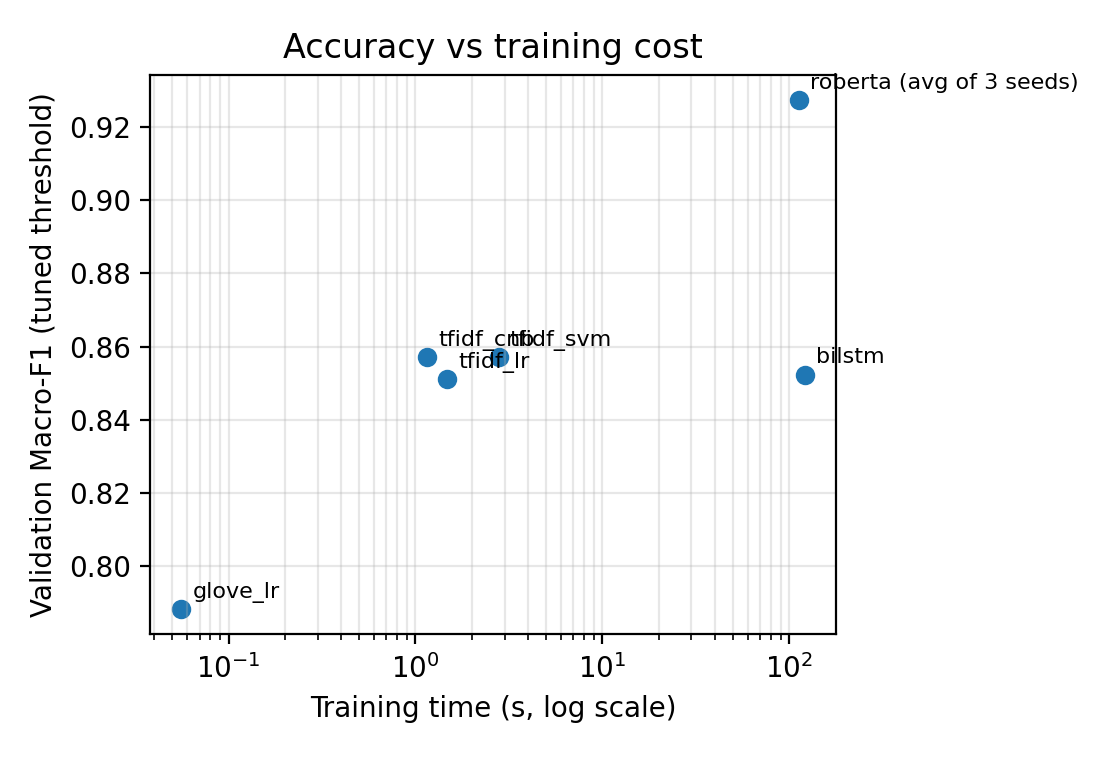
\includegraphics[width=0.62\textwidth]{f1_vs_train_time.png}
\caption{Validation Macro-F1 (tuned threshold) versus training time (log scale). Regenerated by \texttt{src/resource\_table.py} from every model's \texttt{metrics.json}. \tbd{final version after all outputs are in}}
\label{fig:g-scatter}
\end{figure}

\paragraph{Practical implications.}
\begin{itemize}
  \item \textbf{Small labelled data favours pre-trained features.} With only 5.9k training reviews, TF-IDF must learn every n-gram's polarity from scratch, and 24\% of the word types in the validation reviews never occur in training. Pre-trained embeddings, and above all pre-trained language models, bring knowledge learned from billions of words, so they generalise better to rare words, typos and paraphrases.
  \item \textbf{Large data or tight budgets favour sparse features.} TF-IDF scales linearly, runs on any CPU and is fully interpretable. It is the right choice when latency, cost or explainability matter more than the last percentage point, and it is a strong baseline.
  \item \textbf{Robustness to domain change differs.} TF-IDF and GloVe fix their vocabulary at training time. A subword model covers any input string, which matters for the hotel-review scenario in (h).
\end{itemize}
In short, for this task the feature format moves accuracy by a few points but cost by orders of magnitude. The choice should therefore follow the accuracy target and the available hardware.
